%%%%%%%%%%%%%%%%%%%%%%%%%%%%%%%%%%%%%%%%%%%
%%%%%%  STYLE 05
%%%%%%%%%%%%%%%%%%%%%%%%%%%%%%%%%%%%%%%%%%%


\cxset{style05/.style={
 name={Chapter},
 numbering=arabic,
 number font-size=\Large,
 number font-family=\rmfamily,
 number font-weight=\normalfont\itshape,
 number color=\color{black!90},
 number before=,
 number dot=,
 number after=,
 number position=rightname,
 chapter font-family=\rmfamily,
 chapter font-weight=\normalfont\itshape,
 chapter font-size=\Large,
 chapter before={\hrule width \columnwidth \kern2.6pt \par\hfill},
 chapter after={\hfill\hfill\par},
 chapter color={black!90},
 chapter spaceout=none,
 title beforeskip={\vspace*{10pt}},
 title afterskip={\vspace*{50pt}\par},
 title before={\hfill},
 title after={\hfill\hfill \vskip2.6pt\hrule width \columnwidth \kern2.6pt },
 title font-family=\rmfamily,
 title font-color=\color{black!90},
 title font-weight=\bfseries,
 title font-size=\huge,
 header style= headings}}

\cxset{style05}
\chapter{Introduction to Style Five}\index{ch:style5}

\tcbset{width=\textwidth}
I think this style can be improved with a bit of color. You can experiment with it quite easily. The spacing on top of this style can also be adjusted to suit your typographical taste.
\medskip
\begin{figure}[ht]
\centering
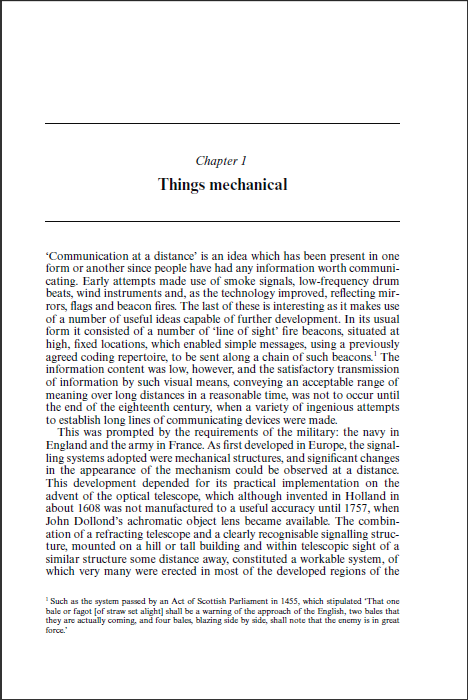
\includegraphics[width=0.6\textwidth]{./chapters/chapter05}
\end{figure}

%\section{General notes on rules}

LaTeX's default rules would normally give problems. Best is to use TeX's primitives to built them.

%\index{rules!example color}
%\begin{texexample}{}{}
%\makeatletter
%\hrule width 5cm \kern2.6\p@
%AAAAAAAAAAAAAAAAAAAAA
%\vskip2.6pt\hrule width 5cm
%\medskip
%
%Problem with LaTeX rules.
%
%\rule{5cm}{0.4pt}\par
%AAAAAAAAAAAAAAAAAAAAA\par%
%\rule[6.5pt]{5cm}{0.4pt}
%
%\def\rule{\@ifnextchar[\@rule{\@rule[\z@]}}
%\def\@rule[#1]#2#3{%
% \leavevmode
% \hbox{%
% \setlength\@tempdima{#1}%
% \setlength\@tempdimb{#2}%
% \setlength\@tempdimc{#3}%
% \advance\@tempdimc\@tempdima%
% \vrule\@width\@tempdimb\@height\@tempdimc\@depth-\@tempdima}}
%
%\def\thickrule{\leavevmode \leaders \hrule height 3pt \hfill \kern \z@}
%
%{\color{teal}\hrule width 10.5cm height3pt \kern2.6\p@
%    {{\color{black!80}\HUGE CHAPTER TITLE}}\vskip3pt
%\hrule width 10.5cm height3pt}
%\makeatother
%\end{texexample}
